% Options for packages loaded elsewhere
\PassOptionsToPackage{unicode}{hyperref}
\PassOptionsToPackage{hyphens}{url}
%
\documentclass[
]{article}
\usepackage{amsmath,amssymb}
\usepackage{iftex}
\ifPDFTeX
  \usepackage[T1]{fontenc}
  \usepackage[utf8]{inputenc}
  \usepackage{textcomp} % provide euro and other symbols
\else % if luatex or xetex
  \usepackage{unicode-math} % this also loads fontspec
  \defaultfontfeatures{Scale=MatchLowercase}
  \defaultfontfeatures[\rmfamily]{Ligatures=TeX,Scale=1}
\fi
\usepackage{lmodern}
\ifPDFTeX\else
  % xetex/luatex font selection
\fi
% Use upquote if available, for straight quotes in verbatim environments
\IfFileExists{upquote.sty}{\usepackage{upquote}}{}
\IfFileExists{microtype.sty}{% use microtype if available
  \usepackage[]{microtype}
  \UseMicrotypeSet[protrusion]{basicmath} % disable protrusion for tt fonts
}{}
\makeatletter
\@ifundefined{KOMAClassName}{% if non-KOMA class
  \IfFileExists{parskip.sty}{%
    \usepackage{parskip}
  }{% else
    \setlength{\parindent}{0pt}
    \setlength{\parskip}{6pt plus 2pt minus 1pt}}
}{% if KOMA class
  \KOMAoptions{parskip=half}}
\makeatother
\usepackage{xcolor}
\usepackage[margin=1in]{geometry}
\usepackage{color}
\usepackage{fancyvrb}
\newcommand{\VerbBar}{|}
\newcommand{\VERB}{\Verb[commandchars=\\\{\}]}
\DefineVerbatimEnvironment{Highlighting}{Verbatim}{commandchars=\\\{\}}
% Add ',fontsize=\small' for more characters per line
\usepackage{framed}
\definecolor{shadecolor}{RGB}{248,248,248}
\newenvironment{Shaded}{\begin{snugshade}}{\end{snugshade}}
\newcommand{\AlertTok}[1]{\textcolor[rgb]{0.94,0.16,0.16}{#1}}
\newcommand{\AnnotationTok}[1]{\textcolor[rgb]{0.56,0.35,0.01}{\textbf{\textit{#1}}}}
\newcommand{\AttributeTok}[1]{\textcolor[rgb]{0.13,0.29,0.53}{#1}}
\newcommand{\BaseNTok}[1]{\textcolor[rgb]{0.00,0.00,0.81}{#1}}
\newcommand{\BuiltInTok}[1]{#1}
\newcommand{\CharTok}[1]{\textcolor[rgb]{0.31,0.60,0.02}{#1}}
\newcommand{\CommentTok}[1]{\textcolor[rgb]{0.56,0.35,0.01}{\textit{#1}}}
\newcommand{\CommentVarTok}[1]{\textcolor[rgb]{0.56,0.35,0.01}{\textbf{\textit{#1}}}}
\newcommand{\ConstantTok}[1]{\textcolor[rgb]{0.56,0.35,0.01}{#1}}
\newcommand{\ControlFlowTok}[1]{\textcolor[rgb]{0.13,0.29,0.53}{\textbf{#1}}}
\newcommand{\DataTypeTok}[1]{\textcolor[rgb]{0.13,0.29,0.53}{#1}}
\newcommand{\DecValTok}[1]{\textcolor[rgb]{0.00,0.00,0.81}{#1}}
\newcommand{\DocumentationTok}[1]{\textcolor[rgb]{0.56,0.35,0.01}{\textbf{\textit{#1}}}}
\newcommand{\ErrorTok}[1]{\textcolor[rgb]{0.64,0.00,0.00}{\textbf{#1}}}
\newcommand{\ExtensionTok}[1]{#1}
\newcommand{\FloatTok}[1]{\textcolor[rgb]{0.00,0.00,0.81}{#1}}
\newcommand{\FunctionTok}[1]{\textcolor[rgb]{0.13,0.29,0.53}{\textbf{#1}}}
\newcommand{\ImportTok}[1]{#1}
\newcommand{\InformationTok}[1]{\textcolor[rgb]{0.56,0.35,0.01}{\textbf{\textit{#1}}}}
\newcommand{\KeywordTok}[1]{\textcolor[rgb]{0.13,0.29,0.53}{\textbf{#1}}}
\newcommand{\NormalTok}[1]{#1}
\newcommand{\OperatorTok}[1]{\textcolor[rgb]{0.81,0.36,0.00}{\textbf{#1}}}
\newcommand{\OtherTok}[1]{\textcolor[rgb]{0.56,0.35,0.01}{#1}}
\newcommand{\PreprocessorTok}[1]{\textcolor[rgb]{0.56,0.35,0.01}{\textit{#1}}}
\newcommand{\RegionMarkerTok}[1]{#1}
\newcommand{\SpecialCharTok}[1]{\textcolor[rgb]{0.81,0.36,0.00}{\textbf{#1}}}
\newcommand{\SpecialStringTok}[1]{\textcolor[rgb]{0.31,0.60,0.02}{#1}}
\newcommand{\StringTok}[1]{\textcolor[rgb]{0.31,0.60,0.02}{#1}}
\newcommand{\VariableTok}[1]{\textcolor[rgb]{0.00,0.00,0.00}{#1}}
\newcommand{\VerbatimStringTok}[1]{\textcolor[rgb]{0.31,0.60,0.02}{#1}}
\newcommand{\WarningTok}[1]{\textcolor[rgb]{0.56,0.35,0.01}{\textbf{\textit{#1}}}}
\usepackage{longtable,booktabs,array}
\usepackage{calc} % for calculating minipage widths
% Correct order of tables after \paragraph or \subparagraph
\usepackage{etoolbox}
\makeatletter
\patchcmd\longtable{\par}{\if@noskipsec\mbox{}\fi\par}{}{}
\makeatother
% Allow footnotes in longtable head/foot
\IfFileExists{footnotehyper.sty}{\usepackage{footnotehyper}}{\usepackage{footnote}}
\makesavenoteenv{longtable}
\usepackage{graphicx}
\makeatletter
\def\maxwidth{\ifdim\Gin@nat@width>\linewidth\linewidth\else\Gin@nat@width\fi}
\def\maxheight{\ifdim\Gin@nat@height>\textheight\textheight\else\Gin@nat@height\fi}
\makeatother
% Scale images if necessary, so that they will not overflow the page
% margins by default, and it is still possible to overwrite the defaults
% using explicit options in \includegraphics[width, height, ...]{}
\setkeys{Gin}{width=\maxwidth,height=\maxheight,keepaspectratio}
% Set default figure placement to htbp
\makeatletter
\def\fps@figure{htbp}
\makeatother
\setlength{\emergencystretch}{3em} % prevent overfull lines
\providecommand{\tightlist}{%
  \setlength{\itemsep}{0pt}\setlength{\parskip}{0pt}}
\setcounter{secnumdepth}{-\maxdimen} % remove section numbering
\ifLuaTeX
  \usepackage{selnolig}  % disable illegal ligatures
\fi
\IfFileExists{bookmark.sty}{\usepackage{bookmark}}{\usepackage{hyperref}}
\IfFileExists{xurl.sty}{\usepackage{xurl}}{} % add URL line breaks if available
\urlstyle{same}
\hypersetup{
  hidelinks,
  pdfcreator={LaTeX via pandoc}}

\author{}
\date{\vspace{-2.5em}}

\begin{document}

\begin{Shaded}
\begin{Highlighting}[]
\FunctionTok{library}\NormalTok{(ggplot2) }\CommentTok{\# Sert à importer ggplot2 pour avoir plusieurs plots}
\FunctionTok{library}\NormalTok{(dplyr)}
\end{Highlighting}
\end{Shaded}

\begin{verbatim}
## 
## Attaching package: 'dplyr'
\end{verbatim}

\begin{verbatim}
## The following objects are masked from 'package:stats':
## 
##     filter, lag
\end{verbatim}

\begin{verbatim}
## The following objects are masked from 'package:base':
## 
##     intersect, setdiff, setequal, union
\end{verbatim}

\begin{Shaded}
\begin{Highlighting}[]
\FunctionTok{library}\NormalTok{(coin)}
\end{Highlighting}
\end{Shaded}

\begin{verbatim}
## Loading required package: survival
\end{verbatim}

\begin{Shaded}
\begin{Highlighting}[]
\CommentTok{\#initialisation}
\FunctionTok{source}\NormalTok{(}\StringTok{"charger.R"}\NormalTok{)}
\NormalTok{mondata }\OtherTok{\textless{}{-}} \FunctionTok{charger}\NormalTok{(}\DecValTok{2212435}\NormalTok{)}
\end{Highlighting}
\end{Shaded}

\hypertarget{phase-1}{%
\subsection{Phase 1:}\label{phase-1}}

\hypertarget{partie-a}{%
\subsubsection{Partie a)}\label{partie-a}}

\begin{Shaded}
\begin{Highlighting}[]
\CommentTok{\#Histogramme}
\NormalTok{h }\OtherTok{\textless{}{-}}\FunctionTok{hist}\NormalTok{(mondata}\SpecialCharTok{$}\NormalTok{IR, }\AttributeTok{main =} \FunctionTok{paste}\NormalTok{(}\StringTok{"Histogramme de l\textquotesingle{}indice de rugosité"}\NormalTok{), }\AttributeTok{col =} \StringTok{"lightpink"}\NormalTok{, }\AttributeTok{xlab =} \StringTok{" Indice de rugosité (sans unité)"}\NormalTok{, }\AttributeTok{ylab =} \StringTok{"Fréquence"}\NormalTok{, }\AttributeTok{xlim =} \FunctionTok{c}\NormalTok{(}\DecValTok{0}\NormalTok{,}\DecValTok{30}\NormalTok{), }\AttributeTok{ylim =} \FunctionTok{c}\NormalTok{(}\DecValTok{0}\NormalTok{,}\DecValTok{50}\NormalTok{))}
\FunctionTok{text}\NormalTok{(h}\SpecialCharTok{$}\NormalTok{mids,h}\SpecialCharTok{$}\NormalTok{counts,}\AttributeTok{labels=}\NormalTok{h}\SpecialCharTok{$}\NormalTok{counts, }\AttributeTok{adj=}\FunctionTok{c}\NormalTok{(}\FloatTok{0.5}\NormalTok{, }\SpecialCharTok{{-}}\FloatTok{0.5}\NormalTok{))}
\end{Highlighting}
\end{Shaded}

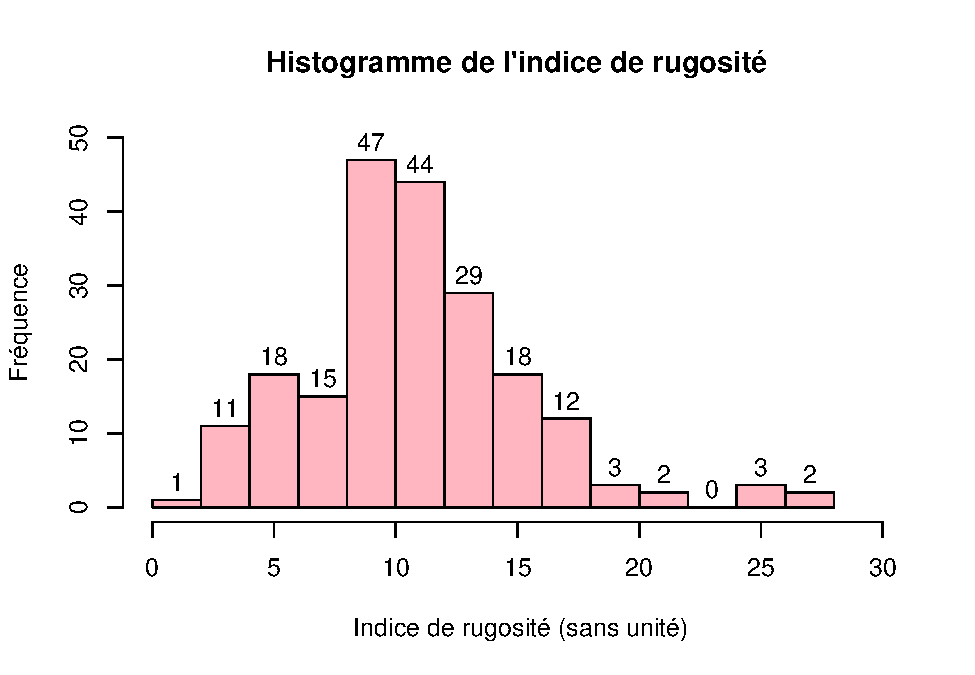
\includegraphics{devoir_files/figure-latex/unnamed-chunk-2-1.pdf}

\begin{Shaded}
\begin{Highlighting}[]
\CommentTok{\#tukey}
\FunctionTok{boxplot}\NormalTok{(mondata}\SpecialCharTok{$}\NormalTok{IR,    }\AttributeTok{main=}\FunctionTok{paste}\NormalTok{(}\StringTok{"Diagramme de tukey de l\textquotesingle{}indice de rugosité"}\NormalTok{),    }\AttributeTok{horizontal=}\NormalTok{T, }\AttributeTok{xlab =} \StringTok{" Indice de rugosité (sans unité)"}\NormalTok{,   }\AttributeTok{col    =}    \StringTok{"lightpink"}\NormalTok{)}
\end{Highlighting}
\end{Shaded}

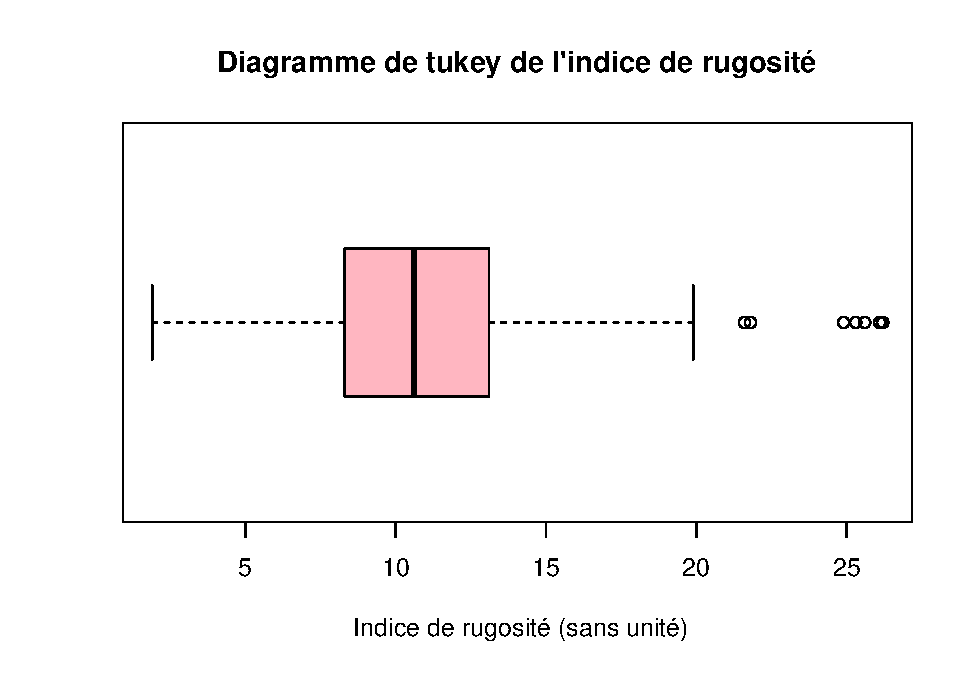
\includegraphics{devoir_files/figure-latex/unnamed-chunk-2-2.pdf}

\begin{Shaded}
\begin{Highlighting}[]
\CommentTok{\#droite de Henry}
\FunctionTok{qqnorm}\NormalTok{(mondata}\SpecialCharTok{$}\NormalTok{IR, }\AttributeTok{col=} \StringTok{"lightpink"}\NormalTok{, }\AttributeTok{main =} \FunctionTok{paste}\NormalTok{(}\StringTok{"Droite de Henry de l\textquotesingle{}indice de rugosité"}\NormalTok{)) }
\FunctionTok{qqline}\NormalTok{(mondata}\SpecialCharTok{$}\NormalTok{IR)}
\end{Highlighting}
\end{Shaded}

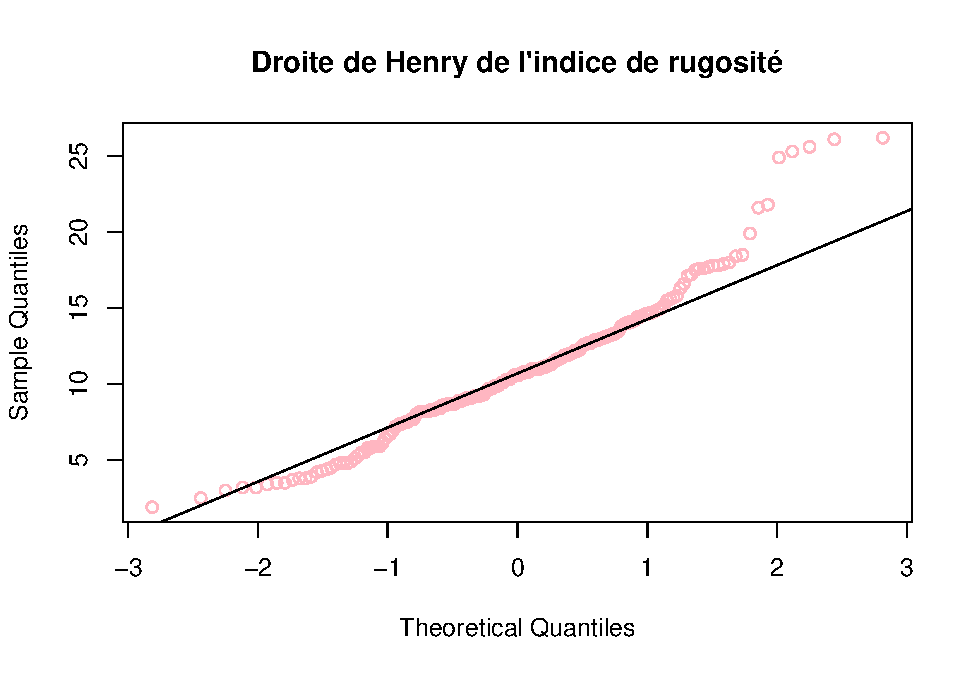
\includegraphics{devoir_files/figure-latex/unnamed-chunk-2-3.pdf}

\begin{Shaded}
\begin{Highlighting}[]
\CommentTok{\#Shapiro}
\FunctionTok{shapiro.test}\NormalTok{(mondata}\SpecialCharTok{$}\NormalTok{IR)}
\end{Highlighting}
\end{Shaded}

\begin{verbatim}
## 
##  Shapiro-Wilk normality test
## 
## data:  mondata$IR
## W = 0.95471, p-value = 4.275e-06
\end{verbatim}

\begin{Shaded}
\begin{Highlighting}[]
\CommentTok{\#tableau statistiques descriptives }

\NormalTok{summary\_table }\OtherTok{\textless{}{-}}\NormalTok{ mondata }\SpecialCharTok{\%\textgreater{}\%}
  \FunctionTok{summarise}\NormalTok{(}
    \AttributeTok{moyenne =} \FunctionTok{mean}\NormalTok{(mondata}\SpecialCharTok{$}\NormalTok{IR),}
    \AttributeTok{ecart\_type\_2 =} \FunctionTok{sd}\NormalTok{(mondata}\SpecialCharTok{$}\NormalTok{IR),}
    \AttributeTok{q1 =} \FunctionTok{quantile}\NormalTok{(mondata}\SpecialCharTok{$}\NormalTok{IR, }\FloatTok{0.25}\NormalTok{),}
    \AttributeTok{q2 =} \FunctionTok{quantile}\NormalTok{(mondata}\SpecialCharTok{$}\NormalTok{IR, }\FloatTok{0.5}\NormalTok{),}
    \AttributeTok{q3 =} \FunctionTok{quantile}\NormalTok{(mondata}\SpecialCharTok{$}\NormalTok{IR, }\FloatTok{0.75}\NormalTok{),}
    \AttributeTok{Interval\_Confiance\_Min =} \FunctionTok{t.test}\NormalTok{(mondata}\SpecialCharTok{$}\NormalTok{IR)}\SpecialCharTok{$}\NormalTok{conf.int[}\DecValTok{1}\NormalTok{],}
    \AttributeTok{Interval\_Confiance\_Max =} \FunctionTok{t.test}\NormalTok{(mondata}\SpecialCharTok{$}\NormalTok{IR)}\SpecialCharTok{$}\NormalTok{conf.int[}\DecValTok{2}\NormalTok{]}
\NormalTok{  )}


\NormalTok{knitr}\SpecialCharTok{::}\FunctionTok{kable}\NormalTok{(summary\_table, }\AttributeTok{caption =} \StringTok{"Tableau des statistiques descriptives sur l\textquotesingle{}indice de rugosité"}\NormalTok{)}
\end{Highlighting}
\end{Shaded}

\begin{longtable}[]{@{}
  >{\raggedleft\arraybackslash}p{(\columnwidth - 12\tabcolsep) * \real{0.1098}}
  >{\raggedleft\arraybackslash}p{(\columnwidth - 12\tabcolsep) * \real{0.1585}}
  >{\raggedleft\arraybackslash}p{(\columnwidth - 12\tabcolsep) * \real{0.0488}}
  >{\raggedleft\arraybackslash}p{(\columnwidth - 12\tabcolsep) * \real{0.0610}}
  >{\raggedleft\arraybackslash}p{(\columnwidth - 12\tabcolsep) * \real{0.0610}}
  >{\raggedleft\arraybackslash}p{(\columnwidth - 12\tabcolsep) * \real{0.2805}}
  >{\raggedleft\arraybackslash}p{(\columnwidth - 12\tabcolsep) * \real{0.2805}}@{}}
\caption{Tableau des statistiques descriptives sur l'indice de
rugosité}\tabularnewline
\toprule\noalign{}
\begin{minipage}[b]{\linewidth}\raggedleft
moyenne
\end{minipage} & \begin{minipage}[b]{\linewidth}\raggedleft
ecart\_type\_2
\end{minipage} & \begin{minipage}[b]{\linewidth}\raggedleft
q1
\end{minipage} & \begin{minipage}[b]{\linewidth}\raggedleft
q2
\end{minipage} & \begin{minipage}[b]{\linewidth}\raggedleft
q3
\end{minipage} & \begin{minipage}[b]{\linewidth}\raggedleft
Interval\_Confiance\_Min
\end{minipage} & \begin{minipage}[b]{\linewidth}\raggedleft
Interval\_Confiance\_Max
\end{minipage} \\
\midrule\noalign{}
\endfirsthead
\toprule\noalign{}
\begin{minipage}[b]{\linewidth}\raggedleft
moyenne
\end{minipage} & \begin{minipage}[b]{\linewidth}\raggedleft
ecart\_type\_2
\end{minipage} & \begin{minipage}[b]{\linewidth}\raggedleft
q1
\end{minipage} & \begin{minipage}[b]{\linewidth}\raggedleft
q2
\end{minipage} & \begin{minipage}[b]{\linewidth}\raggedleft
q3
\end{minipage} & \begin{minipage}[b]{\linewidth}\raggedleft
Interval\_Confiance\_Min
\end{minipage} & \begin{minipage}[b]{\linewidth}\raggedleft
Interval\_Confiance\_Max
\end{minipage} \\
\midrule\noalign{}
\endhead
\bottomrule\noalign{}
\endlastfoot
10.85854 & 4.517969 & 8.3 & 10.6 & 13.1 & 10.23638 & 11.48069 \\
\end{longtable}

\hypertarget{explications}{%
\subsubsection{Explications:}\label{explications}}

L'histogramme de l'indice de rugosité révèle des caractéristiques
significatives sur la distribution de cette mesure au sein de notre
ensemble de données. Deux classes, 8 \textless{} x \textless{} 10 et 10
\textless{} x \textless{} 12, émergent nettement avec les fréquences les
plus élevée, suggérant que la majorité des observations d'IR se
concentrent dans ces plages.De plus, la dispersion des données n'est pas
uniforme, indiquant des concentrations spécifiques plutôt qu'une
répartition égale. Nous pouvons voir avec l'histogramme et le diagramme
de Tukey que les valeurs de l'IR sont assez bien répartie et que les
valeurs sont plus étendues vers la droite, ce qui explique pourquoi la
mediane (q2) est un peu moins élevé que la moyenne. Nous constatons
aussi des données abérantes dans le Diagramme de Tukey. Ces valeurs
aberrantes peuvent avoir un impact sur la moyenne et l'écart-type.C'est
aussi cette distribution anormale (visible à droite de la droite
d'Henry) qui amène les données à échouer le test de normalité. En effet,
le test de Shapiro-Wilk nous donne une valeur p très proche de 0
(4.275e-06), ce qui est inférieur au seuil de 0.05.

\hypertarget{partie-b}{%
\subsubsection{partie b)}\label{partie-b}}

\begin{Shaded}
\begin{Highlighting}[]
\CommentTok{\# sous elements pour les types de M}
\NormalTok{matiere\_A }\OtherTok{\textless{}{-}} \FunctionTok{filter}\NormalTok{(mondata, M }\SpecialCharTok{==} \DecValTok{0}\NormalTok{)}
\NormalTok{matiere\_B }\OtherTok{\textless{}{-}} \FunctionTok{filter}\NormalTok{(mondata, M }\SpecialCharTok{==} \DecValTok{1}\NormalTok{)}

\FunctionTok{layout}\NormalTok{(}\FunctionTok{matrix}\NormalTok{(}\DecValTok{1}\SpecialCharTok{:}\DecValTok{2}\NormalTok{,}\DecValTok{1}\NormalTok{,}\DecValTok{2}\NormalTok{)) }\CommentTok{\# permet de diviser la sortie graphique en deux}
\FunctionTok{hist}\NormalTok{(}\AttributeTok{main =} \FunctionTok{paste}\NormalTok{(}\StringTok{"Histogramme Materiau 0"}\NormalTok{), matiere\_A}\SpecialCharTok{$}\NormalTok{IR, }\AttributeTok{col=}\StringTok{"black"}\NormalTok{,}\AttributeTok{border=}\StringTok{"white"}\NormalTok{,}\AttributeTok{xlab=}\StringTok{"Indice de rugosité"}\NormalTok{,}\AttributeTok{ylab=}\StringTok{"Fréquences"}\NormalTok{)}
\FunctionTok{hist}\NormalTok{(matiere\_B}\SpecialCharTok{$}\NormalTok{IR, }\AttributeTok{col=}\StringTok{"lightpink"}\NormalTok{,}\AttributeTok{border=}\StringTok{"black"}\NormalTok{,}
\AttributeTok{main=}\FunctionTok{paste}\NormalTok{(}\StringTok{"Histogramme Materiau 1"}\NormalTok{),}\AttributeTok{xlab=}\StringTok{"Indice de rugosité"}\NormalTok{,}\AttributeTok{ylab=}\StringTok{"Fréquences"}\NormalTok{)}
\end{Highlighting}
\end{Shaded}

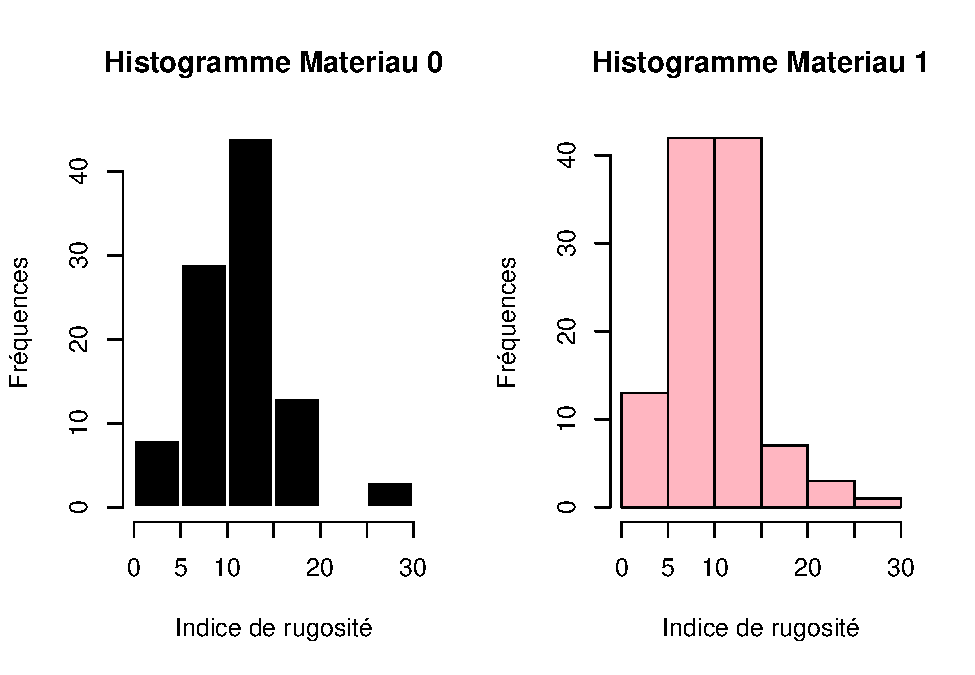
\includegraphics{devoir_files/figure-latex/unnamed-chunk-3-1.pdf}

\begin{Shaded}
\begin{Highlighting}[]
\CommentTok{\#Diagramme de Tukey}
\FunctionTok{ggplot}\NormalTok{(mondata, }\FunctionTok{aes}\NormalTok{(}\AttributeTok{y =} \FunctionTok{factor}\NormalTok{(M), }\AttributeTok{x =}\NormalTok{ IR, }\AttributeTok{fill =} \FunctionTok{factor}\NormalTok{(M))) }\SpecialCharTok{+} \FunctionTok{geom\_boxplot}\NormalTok{(}\AttributeTok{fill =} \FunctionTok{c}\NormalTok{(}\StringTok{"black"}\NormalTok{, }\StringTok{"lightpink"}\NormalTok{))}\SpecialCharTok{+} \FunctionTok{labs}\NormalTok{(}\AttributeTok{fill =} \StringTok{"Materiau"}\NormalTok{,}\AttributeTok{title =} \StringTok{"Diagramme de Tukey de l\textquotesingle{}IR par type de Materiau"}\NormalTok{, }\AttributeTok{y =} \StringTok{"type de Materiau"}\NormalTok{, }\AttributeTok{x =} \StringTok{"indice de Rugosite"}\NormalTok{)}
\end{Highlighting}
\end{Shaded}

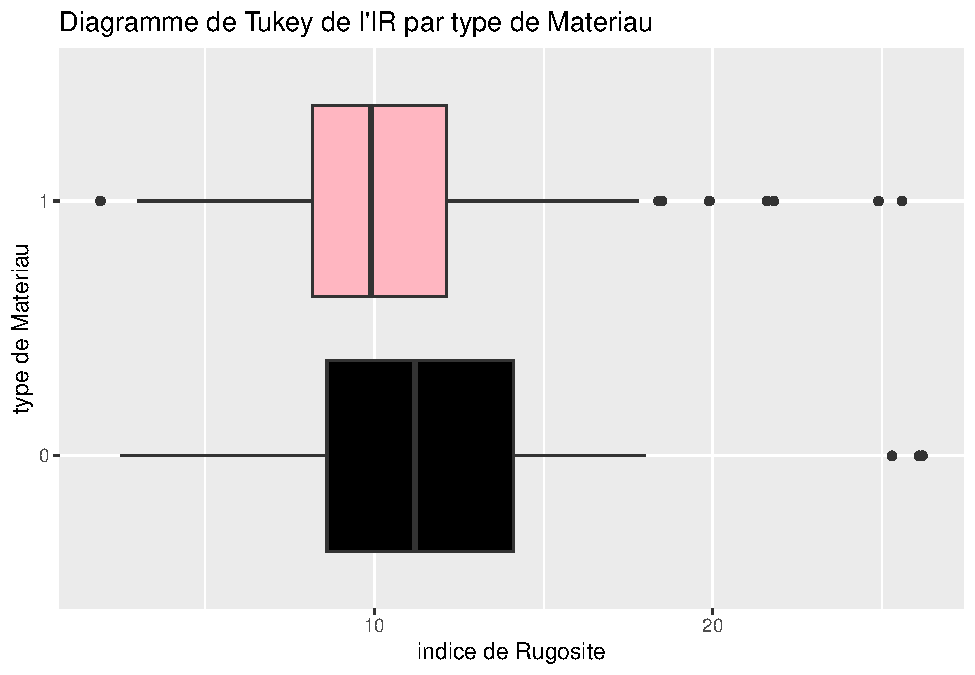
\includegraphics{devoir_files/figure-latex/unnamed-chunk-3-2.pdf}

\begin{Shaded}
\begin{Highlighting}[]
\CommentTok{\#tableau des statistiques descriptives par groupe}
\NormalTok{summary\_table }\OtherTok{\textless{}{-}}\NormalTok{ mondata }\SpecialCharTok{\%\textgreater{}\%}
  \FunctionTok{group\_by}\NormalTok{(M) }\SpecialCharTok{\%\textgreater{}\%}
  \FunctionTok{summarise}\NormalTok{(}
    \AttributeTok{moyenne =} \FunctionTok{mean}\NormalTok{(IR),}
    \AttributeTok{ecart\_type\_2 =} \FunctionTok{sd}\NormalTok{(IR),}
    \AttributeTok{q1 =} \FunctionTok{quantile}\NormalTok{(IR, }\FloatTok{0.25}\NormalTok{),}
    \AttributeTok{q2 =} \FunctionTok{quantile}\NormalTok{(IR, }\FloatTok{0.5}\NormalTok{),}
    \AttributeTok{q3 =} \FunctionTok{quantile}\NormalTok{(IR, }\FloatTok{0.75}\NormalTok{),}
    \AttributeTok{Interval\_Confiance\_Min =} \FunctionTok{t.test}\NormalTok{(IR)}\SpecialCharTok{$}\NormalTok{conf.int[}\DecValTok{1}\NormalTok{],}
    \AttributeTok{Interval\_Confiance\_Max =} \FunctionTok{t.test}\NormalTok{(IR)}\SpecialCharTok{$}\NormalTok{conf.int[}\DecValTok{2}\NormalTok{]}
\NormalTok{  )}


\NormalTok{knitr}\SpecialCharTok{::}\FunctionTok{kable}\NormalTok{(summary\_table, }\AttributeTok{caption =} \StringTok{"Tableau des statistiques descriptives sur l\textquotesingle{}indice de rugosité pour le materiau 1 et 0"}\NormalTok{)}
\end{Highlighting}
\end{Shaded}

\begin{longtable}[]{@{}
  >{\raggedleft\arraybackslash}p{(\columnwidth - 14\tabcolsep) * \real{0.0337}}
  >{\raggedleft\arraybackslash}p{(\columnwidth - 14\tabcolsep) * \real{0.1011}}
  >{\raggedleft\arraybackslash}p{(\columnwidth - 14\tabcolsep) * \real{0.1461}}
  >{\raggedleft\arraybackslash}p{(\columnwidth - 14\tabcolsep) * \real{0.0674}}
  >{\raggedleft\arraybackslash}p{(\columnwidth - 14\tabcolsep) * \real{0.0562}}
  >{\raggedleft\arraybackslash}p{(\columnwidth - 14\tabcolsep) * \real{0.0787}}
  >{\raggedleft\arraybackslash}p{(\columnwidth - 14\tabcolsep) * \real{0.2584}}
  >{\raggedleft\arraybackslash}p{(\columnwidth - 14\tabcolsep) * \real{0.2584}}@{}}
\caption{Tableau des statistiques descriptives sur l'indice de rugosité
pour le materiau 1 et 0}\tabularnewline
\toprule\noalign{}
\begin{minipage}[b]{\linewidth}\raggedleft
M
\end{minipage} & \begin{minipage}[b]{\linewidth}\raggedleft
moyenne
\end{minipage} & \begin{minipage}[b]{\linewidth}\raggedleft
ecart\_type\_2
\end{minipage} & \begin{minipage}[b]{\linewidth}\raggedleft
q1
\end{minipage} & \begin{minipage}[b]{\linewidth}\raggedleft
q2
\end{minipage} & \begin{minipage}[b]{\linewidth}\raggedleft
q3
\end{minipage} & \begin{minipage}[b]{\linewidth}\raggedleft
Interval\_Confiance\_Min
\end{minipage} & \begin{minipage}[b]{\linewidth}\raggedleft
Interval\_Confiance\_Max
\end{minipage} \\
\midrule\noalign{}
\endfirsthead
\toprule\noalign{}
\begin{minipage}[b]{\linewidth}\raggedleft
M
\end{minipage} & \begin{minipage}[b]{\linewidth}\raggedleft
moyenne
\end{minipage} & \begin{minipage}[b]{\linewidth}\raggedleft
ecart\_type\_2
\end{minipage} & \begin{minipage}[b]{\linewidth}\raggedleft
q1
\end{minipage} & \begin{minipage}[b]{\linewidth}\raggedleft
q2
\end{minipage} & \begin{minipage}[b]{\linewidth}\raggedleft
q3
\end{minipage} & \begin{minipage}[b]{\linewidth}\raggedleft
Interval\_Confiance\_Min
\end{minipage} & \begin{minipage}[b]{\linewidth}\raggedleft
Interval\_Confiance\_Max
\end{minipage} \\
\midrule\noalign{}
\endhead
\bottomrule\noalign{}
\endlastfoot
0 & 11.49381 & 4.598071 & 8.600 & 11.2 & 14.100 & 10.567098 &
12.42053 \\
1 & 10.28796 & 4.387849 & 8.175 & 9.9 & 12.125 & 9.450959 & 11.12497 \\
\end{longtable}

\hypertarget{explication}{%
\subsubsection{Explication:}\label{explication}}

Tout d'abord, les histogrammes nous permet de constater que la plupart
des valeurs pour les deux matériaux se situent dans les mêmes classes
(classe 5-10 et classe 10-15), avec des valeurs plus etendues vers la
droite. Les histogrammes et le diagramme nous permettent de constater
que la moyenne du Matériau 0 est plus élevée que celle du Matériau 1 par
leurs distributions. Cette observation est cohérente avec les calculs
des statistiques descriptives. En effet, en examinant les moyennes, le
Matériau 0 affiche une moyenne de 11.49 et de 10.29 pour Matériau 1,
confirmant la tendance constaté. De plus, les quartiles et les
intervalles de confiance décrivent la répartition des données, montrant
que le Matériau 0 a une distribution plus étendue que le Matériau 1.
Cette conclusion est également étayée par l'écart-type, qui est
légèrement plus élevé pour le Matériau 0 (4.60) que pour le Matériau 1
(4.39). Les observations du diagramme de Tukey renforce ces résultats,
suggérant que le centre du Matériau 0 est inférieur à celui du Matériau
1. En résumé, on peut constater des différences entre les deux matériaux
que ce soit de tendance centrale, de dispersion ou de la présence de
données aberrantes.

Avant de procéder aux tests d`hypothèses, nous allons effectuer le test
de shapiro pour verifier si l'échantillon d'IR pour les deux types de
matières suivent une loi normale:

\begin{Shaded}
\begin{Highlighting}[]
\FunctionTok{shapiro.test}\NormalTok{(matiere\_A}\SpecialCharTok{$}\NormalTok{IR)}
\end{Highlighting}
\end{Shaded}

\begin{verbatim}
## 
##  Shapiro-Wilk normality test
## 
## data:  matiere_A$IR
## W = 0.95848, p-value = 0.003767
\end{verbatim}

\begin{Shaded}
\begin{Highlighting}[]
\FunctionTok{shapiro.test}\NormalTok{(matiere\_B}\SpecialCharTok{$}\NormalTok{IR)}
\end{Highlighting}
\end{Shaded}

\begin{verbatim}
## 
##  Shapiro-Wilk normality test
## 
## data:  matiere_B$IR
## W = 0.93804, p-value = 7.851e-05
\end{verbatim}

\hypertarget{tests-dhypothese-moyenne-uxe9gale}{%
\subsubsection{Tests d'hypothese moyenne
égale:}\label{tests-dhypothese-moyenne-uxe9gale}}

Comme la valeur p est inférieure à 0.05 dans les deux cas (0.003767
\textless{} 0.05 et 7.851e-05 \textless\textless\textless{} 0.05), on
rejette l'hypothèse nulle selon laquelle les échantillons suivent une
distribution normale.Nous allons donc utiliser le test de student afin
de vérifier si les deux moyennes sont égales. Voici nos hypothèses:

\(H_0: \mu_1 = \mu_2\) \(H_1: \mu_1 \neq \mu_2\)

Puisque les variances sont inconnues, nous allons utiliser le test de
Student suivant:

\(Z_0 = (\bar{X_1} - \bar{X_2}) / \sqrt[2]{(S_1^2/n_1)+(S_2^2/n_2)}\)

\begin{Shaded}
\begin{Highlighting}[]
\CommentTok{\# test d\textquotesingle{}hypothese:}
\FunctionTok{source}\NormalTok{(}\StringTok{"charger.R"}\NormalTok{)}
\NormalTok{mondata }\OtherTok{\textless{}{-}} \FunctionTok{charger}\NormalTok{(}\DecValTok{2212435}\NormalTok{)}
\NormalTok{matiere\_A }\OtherTok{\textless{}{-}} \FunctionTok{filter}\NormalTok{(mondata, M }\SpecialCharTok{==} \DecValTok{0}\NormalTok{)}
\NormalTok{matiere\_B }\OtherTok{\textless{}{-}} \FunctionTok{filter}\NormalTok{(mondata, M }\SpecialCharTok{==} \DecValTok{1}\NormalTok{)}

\FunctionTok{t.test}\NormalTok{(matiere\_A}\SpecialCharTok{$}\NormalTok{IR,matiere\_B}\SpecialCharTok{$}\NormalTok{IR)}
\end{Highlighting}
\end{Shaded}

\begin{verbatim}
## 
##  Welch Two Sample t-test
## 
## data:  matiere_A$IR and matiere_B$IR
## t = 1.9157, df = 198.26, p-value = 0.05685
## alternative hypothesis: true difference in means is not equal to 0
## 95 percent confidence interval:
##  -0.03546338  2.44716632
## sample estimates:
## mean of x mean of y 
##  11.49381  10.28796
\end{verbatim}

\hypertarget{interpruxe9tation}{%
\subsubsection{Interprétation:}\label{interpruxe9tation}}

Puisque le p-value est suppérieur à 0.05 (0.05685 \textgreater{} 0.05)
donc nous ne pouvons pas rejeter H0 à un niveau de confiance de 95\%. Il
n'y a donc pas suffisamment de preuves statistiques pour affirmer que
les moyennes des deux groupes sont egales.

\end{document}
